\section{Background on Shrimpy}


\begin{frame}
  \frametitle{Outline}
  \tableofcontents[ currentsection ]
\end{frame}

\subsection{The Problem}

\begin{frame}
  \frametitle{The Problem}

  Southern German water routes have had several drastic population
  changes concerning gammarids (Kinzler, 2008) \cite{Dikerogammarus}.

  \vfill

  Much of this is due to canal construction. 

  \begin{columns}[t]
    \column{.45\textwidth} 
	\begin{block}{Native Species:}
    %\centerline{\includegraphics[height=5.0cm]{gainComp-001}} 
	\textit{Gammarus pulex (Gp)}
	\end{block}

    \column{.55\textwidth}
	\begin{block}{Invasive Species:}
    %\centerline{\includegraphics[height=5.0cm]{energyComp-001}}
    	\textit{Dikerogammarus villosus (Dv)}\\	
	\textit{Dikerogammarus haemobaphes (Dh)}\\
	\textit{Dikerogammarus bispinosus (Db)}\\
	\textit{Echinogammarus berilloni (Eb)}
	\end{block}
  \end{columns}
\end{frame}

\begin{frame}{Killer Shrimp}
  \centerline{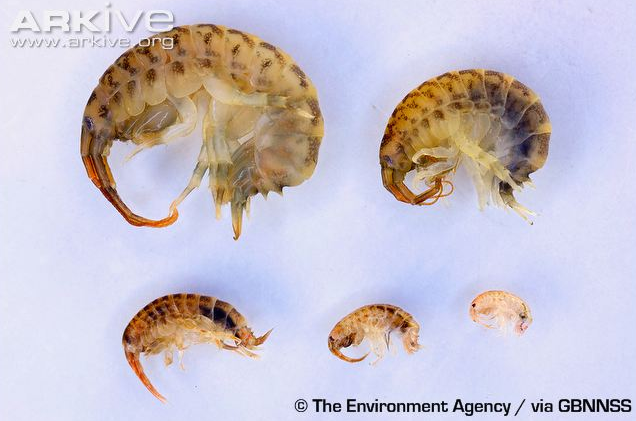
\includegraphics[width=8cm]{img/shrimpy1}}

  \center{http://www.arkive.org/killer-shrimp/dikerogammarus-villosus/image-G143154.html}
\end{frame}

\begin{frame}{Killer Shrimp}
  \centerline{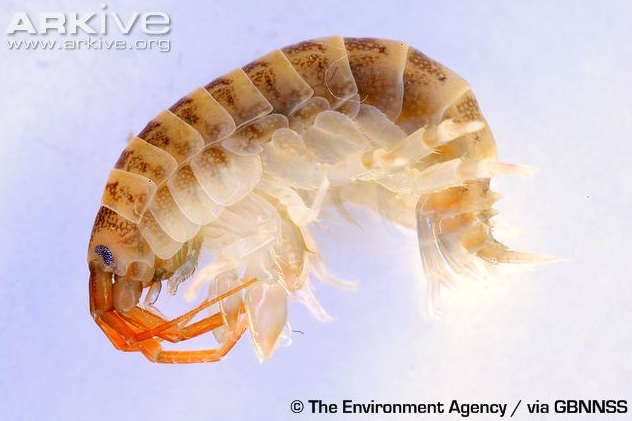
\includegraphics[width=8cm]{img/shrimpy2}}

  \center{http://www.arkive.org/killer-shrimp/dikerogammarus-villosus/image-G143155.html}
\end{frame}

\begin{frame}{Killer Shrimp}
  \centerline{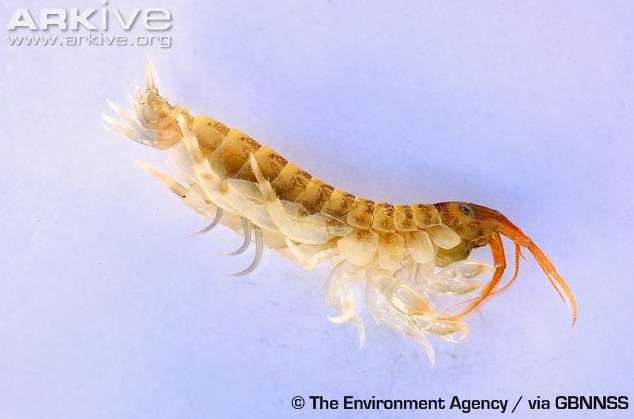
\includegraphics[width=8cm]{img/shrimpy3}}

	\center{http://www.arkive.org/killer-shrimp/dikerogammarus-villosus/image-G143156.html}
\end{frame}

\begin{frame}
	\centerline{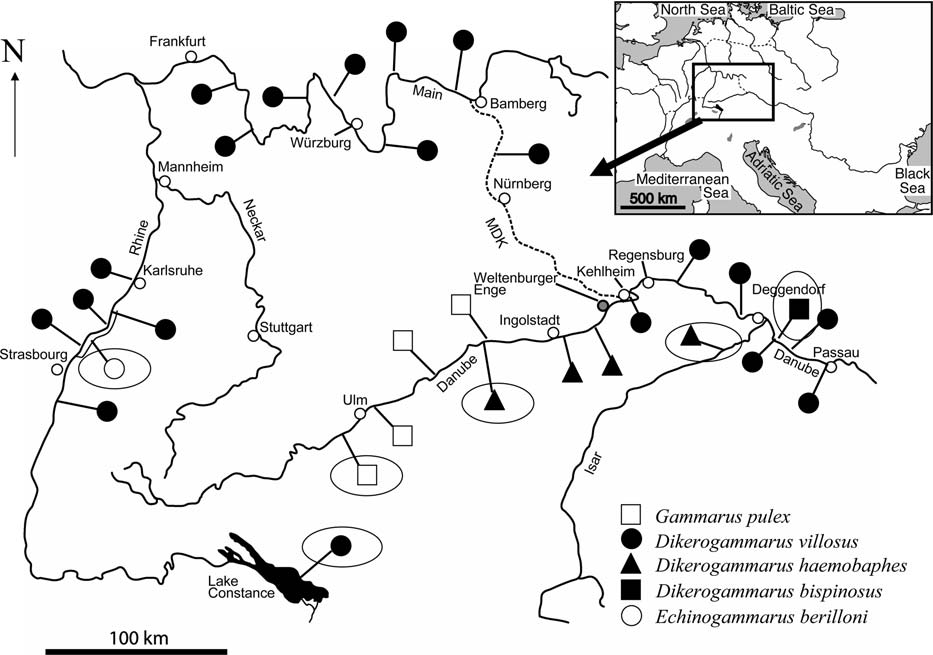
\includegraphics[width=10cm]{img/kinzlermap}}
	
	\center{(Kinzler, 2008)}
\end{frame}


\begin{frame}{Time Line}

  \vfill

  \begin{tabular}{l|l}
    Years      & Species \\ \hline
    $<$1976    & \textit{Gp} native\\
    1976-1994  & \textit{Dh} invades\\
    1992-1995  & \textit{Dv} invades, \textit{Dh} declines\\
    $>$1995    & All but \textit{Dv} coexist separate from \textit{Dv}
  \end{tabular}

  \vfill

\end{frame}


\begin{frame}
   \frametitle{Kinzler, 2008 Study}
	\vfill
	
	Isolated pairs of specimens in a controlled environment
	\begin{itemize}
		\item One freshly moulted (prey) 
		\item One predator
		\item Total of 279 experiments
		\item Grouped by age, sex, and species \**
	\end{itemize}
	
\vfill
	Results\\
\begin{itemize}
	\item Found \textit{Dv} to be clear strongest predator\\
\vspace{.5em}
	\item Found \textit{Dh} to have highest cannibalism rate
\end{itemize}

\vfill

\** Intraguild: predation between different species;\\ 
\hspace{.5em} Intraspecific: predation within species (cannibalism) \cite{doi:10.1146/annurev.es.20.110189.001501}

\end{frame}

\begin{frame}
   \frametitle{Basic Goals}
\begin{center}
		{\Large{\textbf{Determine long term population trends!}}}\\


\vspace{2.5em}
		Does \textit{Dv} totally dominate in the end?\\
\vspace{.5em}
		Which species survive?\\
\vspace{.5em}

		Is there an equilibrium?

\end{center}

\end{frame}


%\begin{frame}
%  \frametitle{The Issues}
%
%  We gonna talk about the issues about talking about stuff.
%
%\end{frame}
%
%
%\begin{frame}
%  \frametitle{Random Stuff}
%
%  Random stuff is like totally out there.
%
%  \uncover<2->
%  {
%
%    It could just be totally surprising.
%
%  }
%
%  \uncover<3->
%  {
%
%    Unexpected even, you know what I mean?
%
%  }
%
%
%\end{frame}
%
%
%\subsection{Statistics}
%
%\begin{frame}{Statistics Do Not Lie}
%
%  You can totally trust the statistics.
%
%  \only<2>{
%
%    Well... usually
%    \begin{itemize}
%    \item We could make a type I error.
%    \item Or it could be a type II error.
%    \end{itemize}
%
%  }
%
%  \only<3-4>{
%
%    Then again maybe the hypothesis test does not even make sense.
%
%  }
%
%  \only<4->{
%
%    Then you are really hosed.
%
%  }
%
%\end{frame}


